\chapter{Estimation \& Planning}
{
	The Gantt Chart below shows a complete timeline this software will undergo during the developmental phase. \\
	\begin{figure}[h]
		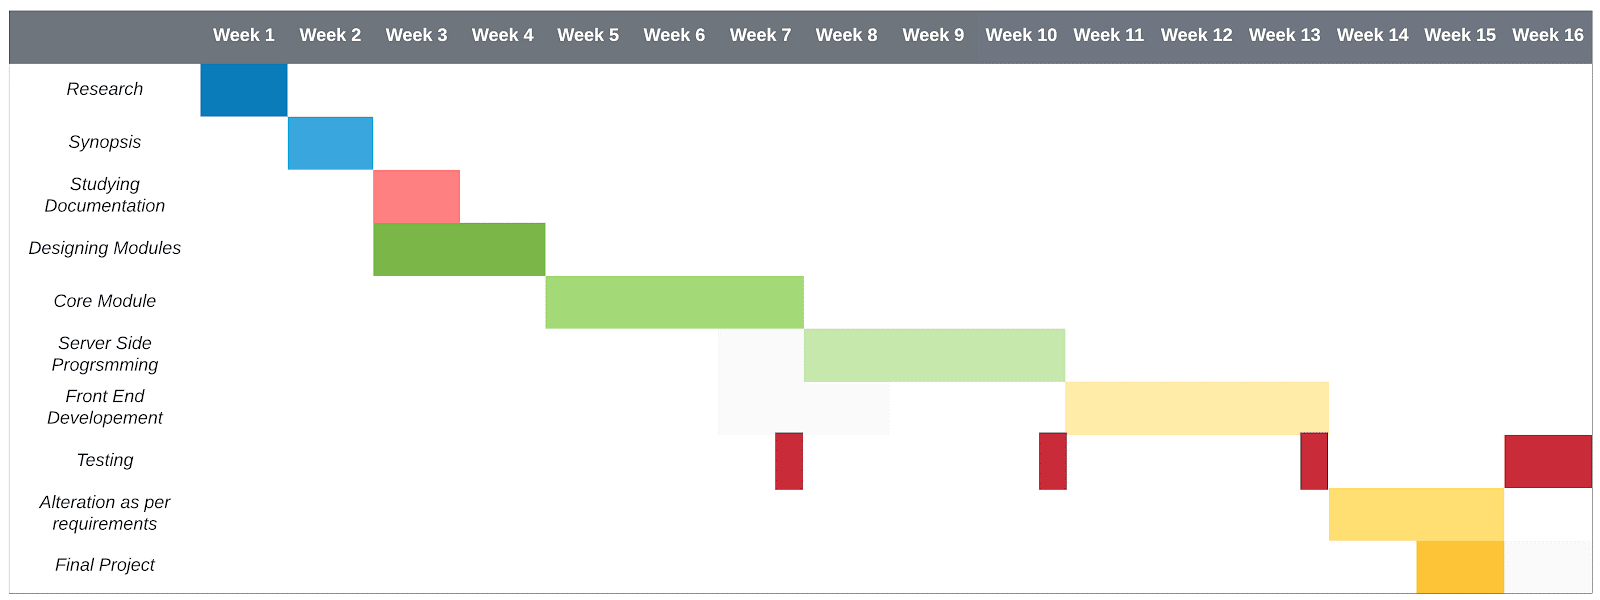
\includegraphics[width=\linewidth,height=10cm]{media/gantt_chart.png}
		\caption{Gantt Chart for project development}
	\end{figure}
	\begin{itemize}
		\item Starting up with the research first week will mark the completion of the research. 
		\item Synopsis will be completed within the second week.
		\item In the third week initial preparation and the documentation of the required libraries will be studied.
		\item Parallelly the modules for the entire website will be designed. Its completion will mark the end of fourth week.
		\item The beginning of fifth week will initiate the coding phase. The Core Module will be completed in 3 weeks of time. At the end of seventh week the testing of Core Module will also be conducted hand in hand.
		\item Server-Side Programming will be started on the eighth week of the timeline. It also will be completed in 3 weeks of time along with its testing.
		\item Eleventh week will start by initiating the coding of Front End. Corresponding testing will be started by the end of thirteenth week, thus, completing the Front-End Development.
		\item Changes, if any, are advised, will be completed during fourteenth and fifteenth week.
		\item The final project will also be completed in the fifteenth week.
		\item The entire project will be tested to ensure an error free software in the sixteenth week.
		\item Thus, the entire software will be developed in 16 weeks of time.
	\end{itemize}
}